\providecommand{\main}{..}

\documentclass[/home/francois/latex/report/main.tex]{subfiles}

\begin{document}

\chapter{Background}
\label{chapter:background}

This chapter introduces the hardware setup, the mechanical models and the mathematical optimization framework that will be the core of the thesis:

\section{Hardware setup}
\label{section:hardware}

Below are described the hardware equipment provided by the host organization. It comprises the robotic arm, the Force/Torque (FT) sensor attached to the last joint, the gripper tool, and its \textit{suction cup}. A typical motion of the robot during \textit{pick-and-place} operation is described. Also, key physical behaviors of the system that influence the design of the mechanical models are highlighted.

\subsection{Robotic manipulator}

Two models of 6 Degrees of Freedom (DoF) robotic arms have been used throughout the project: UR10 and UR10e from \textsc{Universal Robot}\texttrademark \ (cf. Figure \ref{fig:background:stanislaw}). They are fairly similar since they can both span an circular area with radius $1300 \si{\milli\meter}$ around them and handle payloads over $10 \si{\kilo\gram}$ –as suggested by the name. The particularity of UR10e is its built-in \ac{FT} sensor and faster communication ($500 \si{\hertz}$ by contrast with $125 \si{\hertz}$ of the UR10).

\begin{figure}[h]
  \centering
  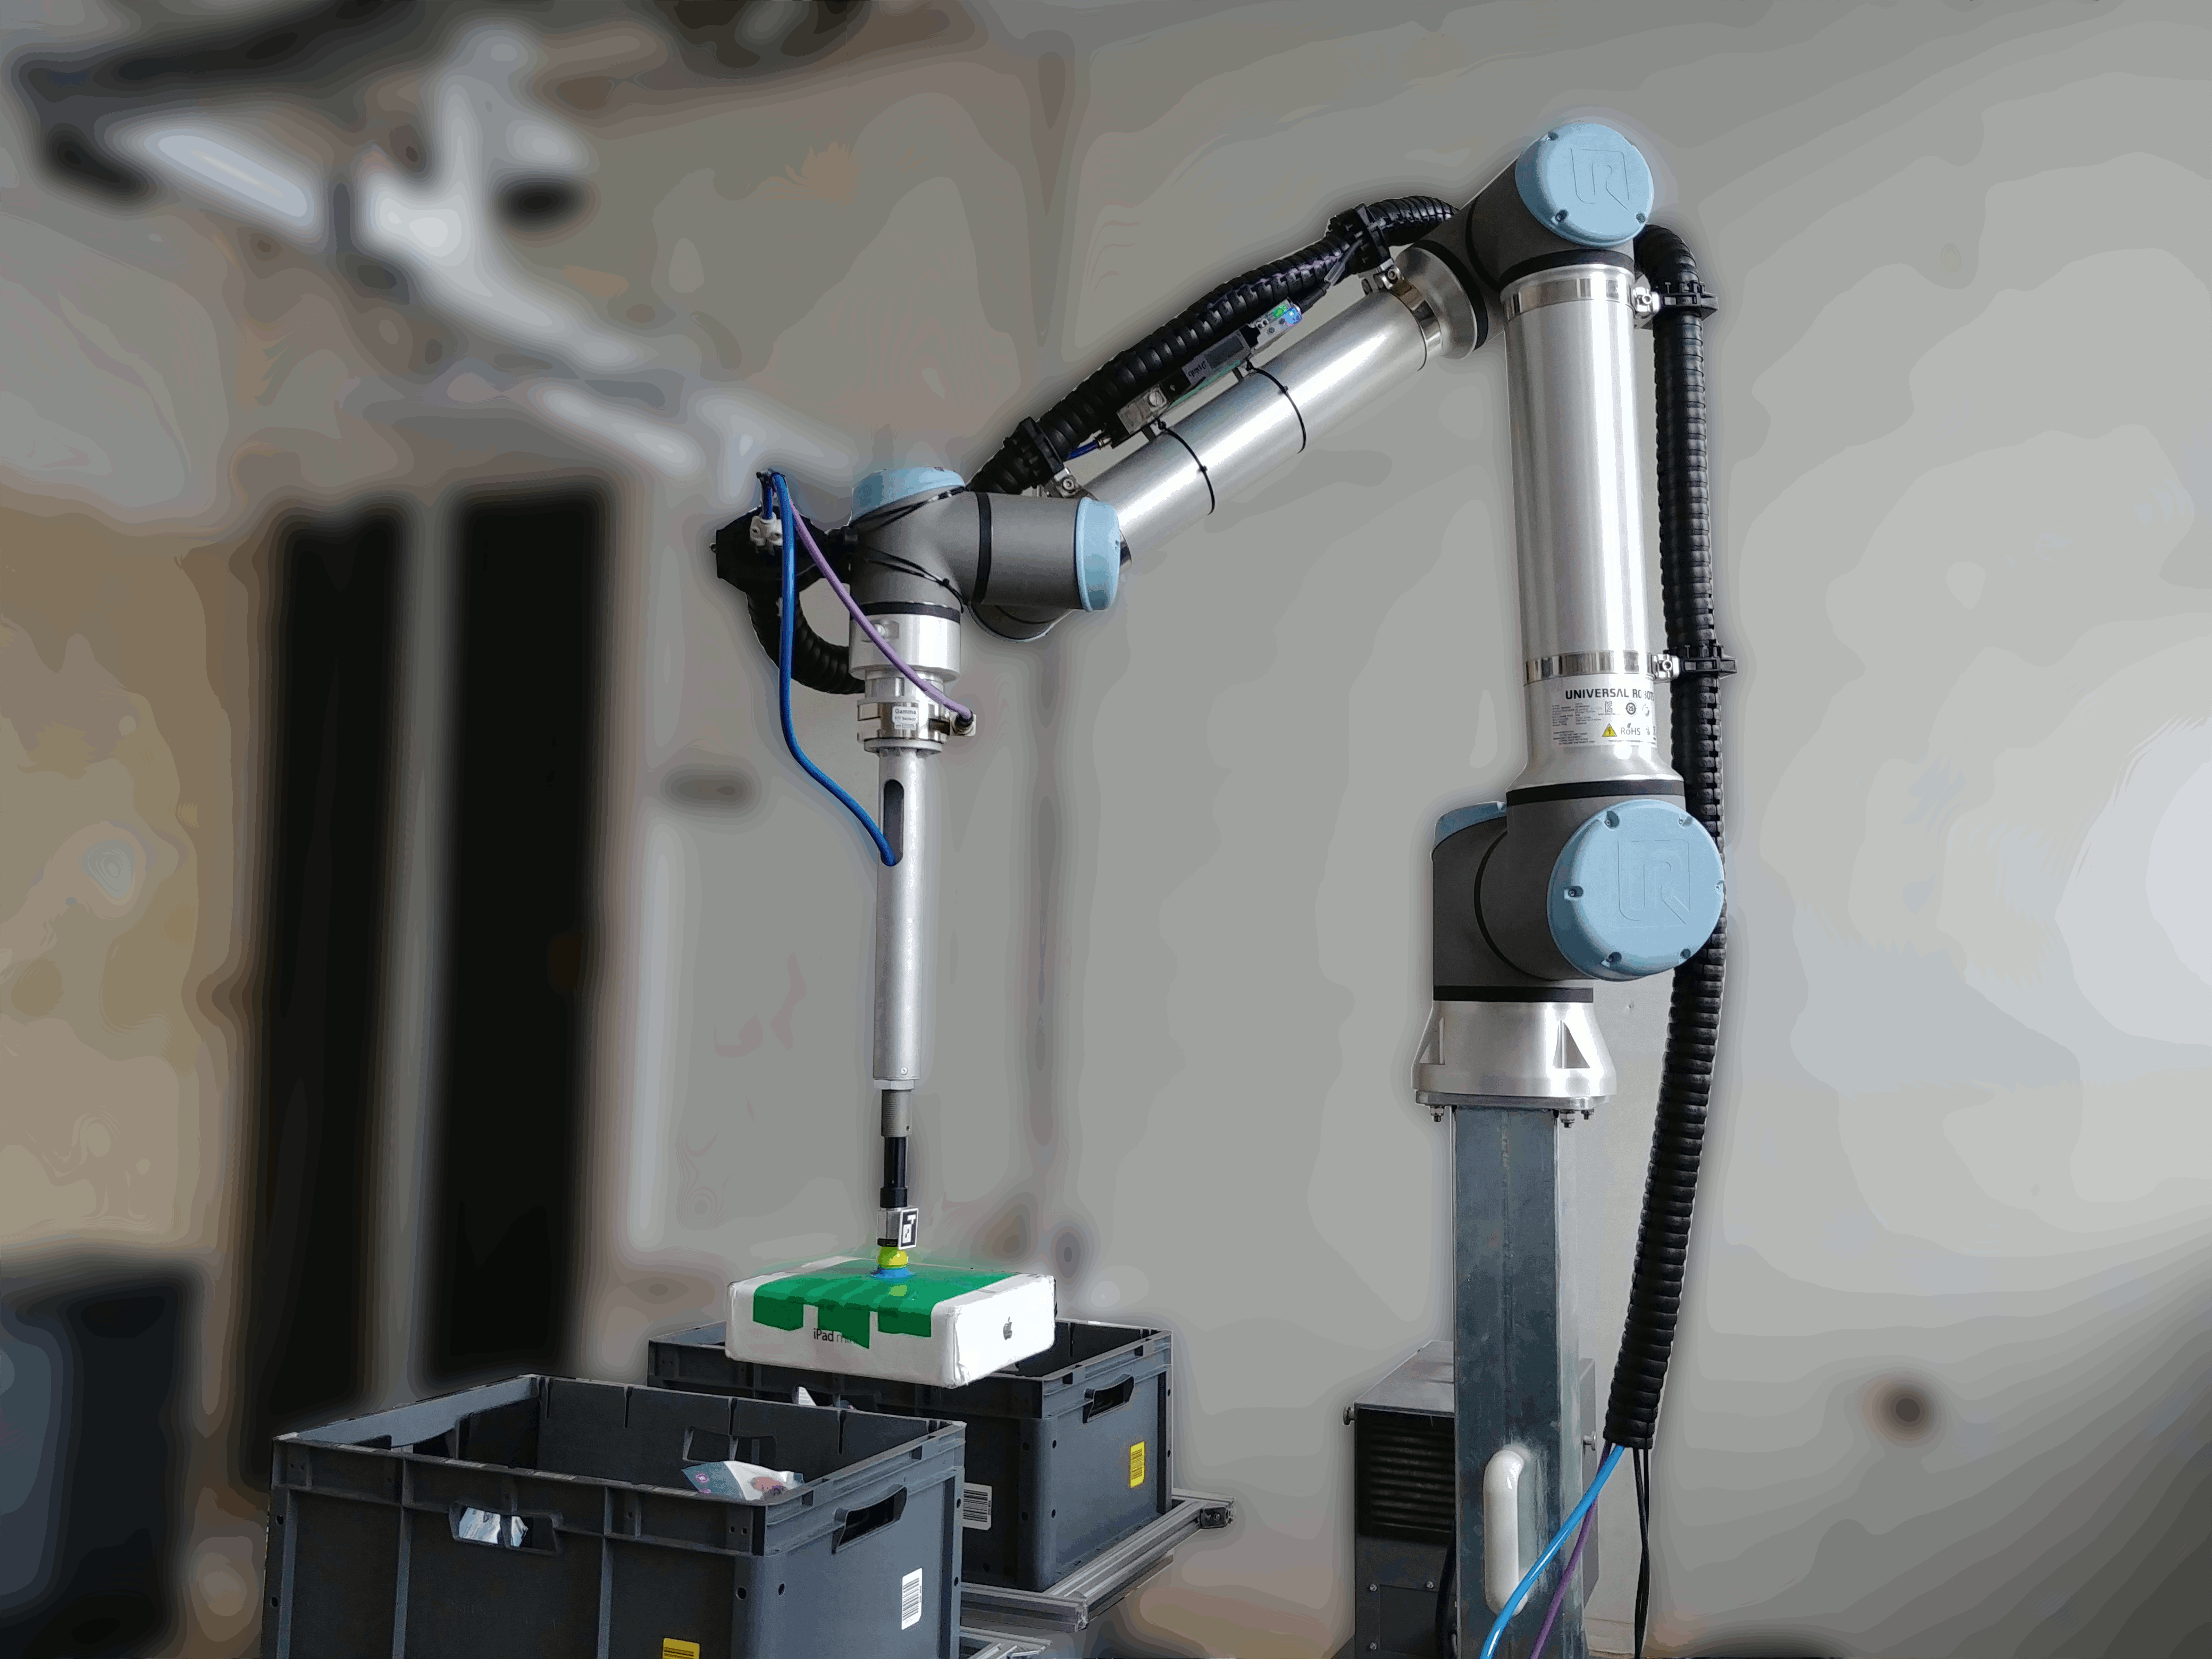
\includegraphics[scale=0.08]{\main/figures/picture_of_ur_indexed.png}
  \caption{Robotic arm from \textsc{Universal Robot}\texttrademark \ grasping an iPad box. The UR10e manipulator is mounted on a base to reach a larger area. The blue cable connect the suction cup to the pneumatic network and the purple cable connect the \ac{FT} sensor to the robot unit. The two totes in the background can be source or target places for \textit{pick-and-place} tasks.}
  \label{fig:background:stanislaw}
\end{figure}

\subsection{\ac{FT} sensor}

Two \ac{FT} sensors are used within the project. The built-in sensor of UR10e and the \textit{Gamma} \ac{FT} sensor from ATI\texttrademark. They are both mounted on the last joint of both robotic manipulators (cf. Figure \ref{fig:background:tool}). The ATI\texttrademark \ sensor is the primary sensor throughout the evaluation of the different approaches. Although its range of measurement is narrower than UR10e one, it has better resolution properties (cf. Table \ref{tab:background:ft-sensor}).

\begin{table}[h]
  \begin{center}
    \renewcommand{\arraystretch}{1.8} % Default value: 1
    \begin{tabular}{l|c|c} % <-- Alignments: 1st column left, 2nd middle and 3rd right, with vertical lines in between
      & \textbf{ATI Gamma} & \textbf{UR10e}\\
      \hline
      Range (force)  & $F_{x/y}: 32 \ \si{\newton}$ $F_z: 100 \ \si{\newton}$ & \underline{$100 \ \si{\newton}$} \\
      \hline
      Range (torque)  & $2.5 \ \si{\newton} \si{\meter}$ & \underline{$10 \ \si{\newton} \si{\meter}$} \\
      \hline
      Resolution (force)  & \underline{$F_{x/y}: 0.0062 \ \si{\newton}$ $F_z: 0.012 \ \si{\newton}$} & $2.0 \ \si{\newton}$ \\
      \hline
      Resolution (torque)  & \underline{$0.0005 \ \si{\newton} \si{\meter}$} & $0.02 \ \si{\newton} \si{\meter}$ \\
      \hline
    \end{tabular}
  \end{center}
  \caption{Specifications of the built-in UR10e sensor and \textit{Gamma} sensor \cite{ati, ur10e}. The \textit{Gamma} sensor offers the possibility to measure at a higher range but with lower resolution. The higher resolution is prefered in this particular case.\label{tab:background:ft-sensor}}
\end{table}

\subsection{End-effector}

The end-effector of the robot fulfills the functions of grasping a wide range of items, measuring the force induced on the wrist, safely picking from diverse source totes, carts or conveyors. It consists of 4 basic elements (cf. Figure \ref{fig:background:tool}):

\begin{itemize}
  \item an ATI\texttrademark \ sensor which is screwed on the wrist of the robotic manipulator,
  \item an extension tube to reach deep totes or carts,
  \item a second cylinder inserted in the previous one with a safety-spring,
  \item a vacuum suction cup linked to the pneumatic supply.
\end{itemize}

\begin{figure}[h]
  \centering
  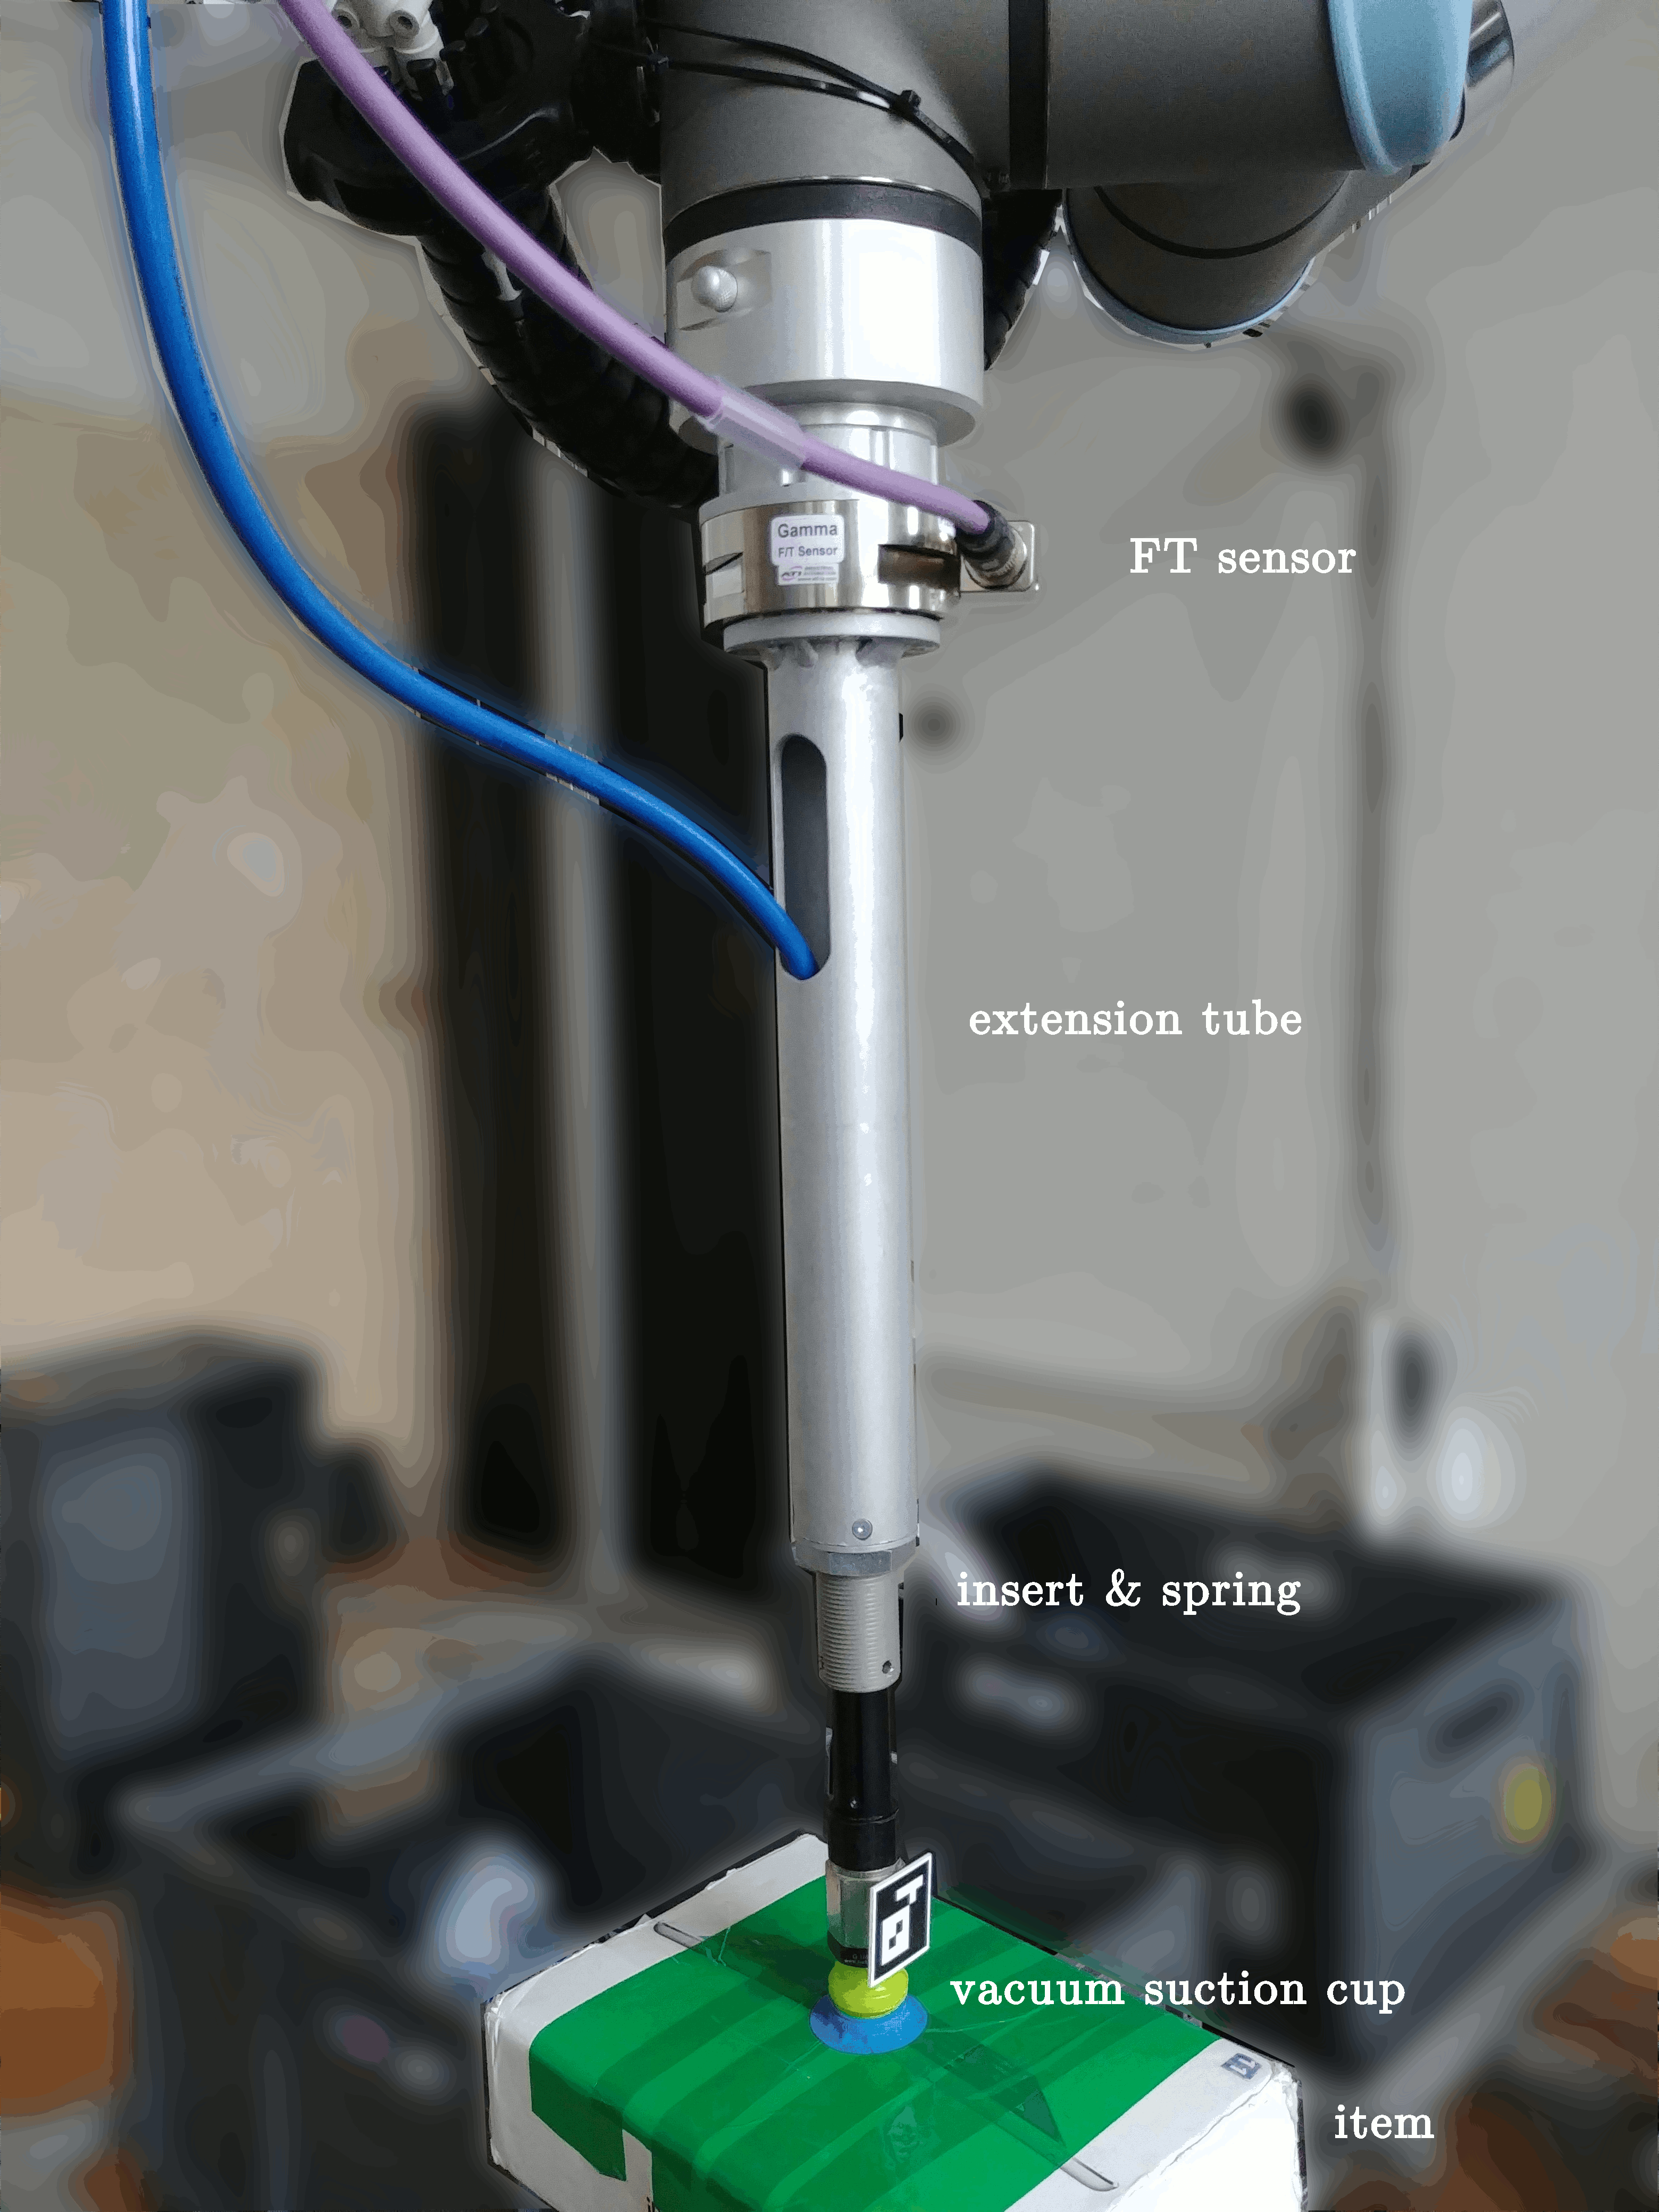
\includegraphics[scale=0.08]{\main/figures/picture_of_tool_indexed.png}
  \caption{Tool mount on the robotic manipulator handling an iPad box. The safety-spring cannot be seen on this picture because it is inside the extension tube.}
  \label{fig:background:tool}
\end{figure}

A suction cup with a springy extension is mounted on the tool. It allows a very simple integration logic and a versatile ability to grasp items (cf. Figure \ref{fig:background:suction}). The sealing lip provides a good grip on a large range of object textures.

\begin{figure}[h]
\centering
\begin{subfigure}{0.49\textwidth}
\centering
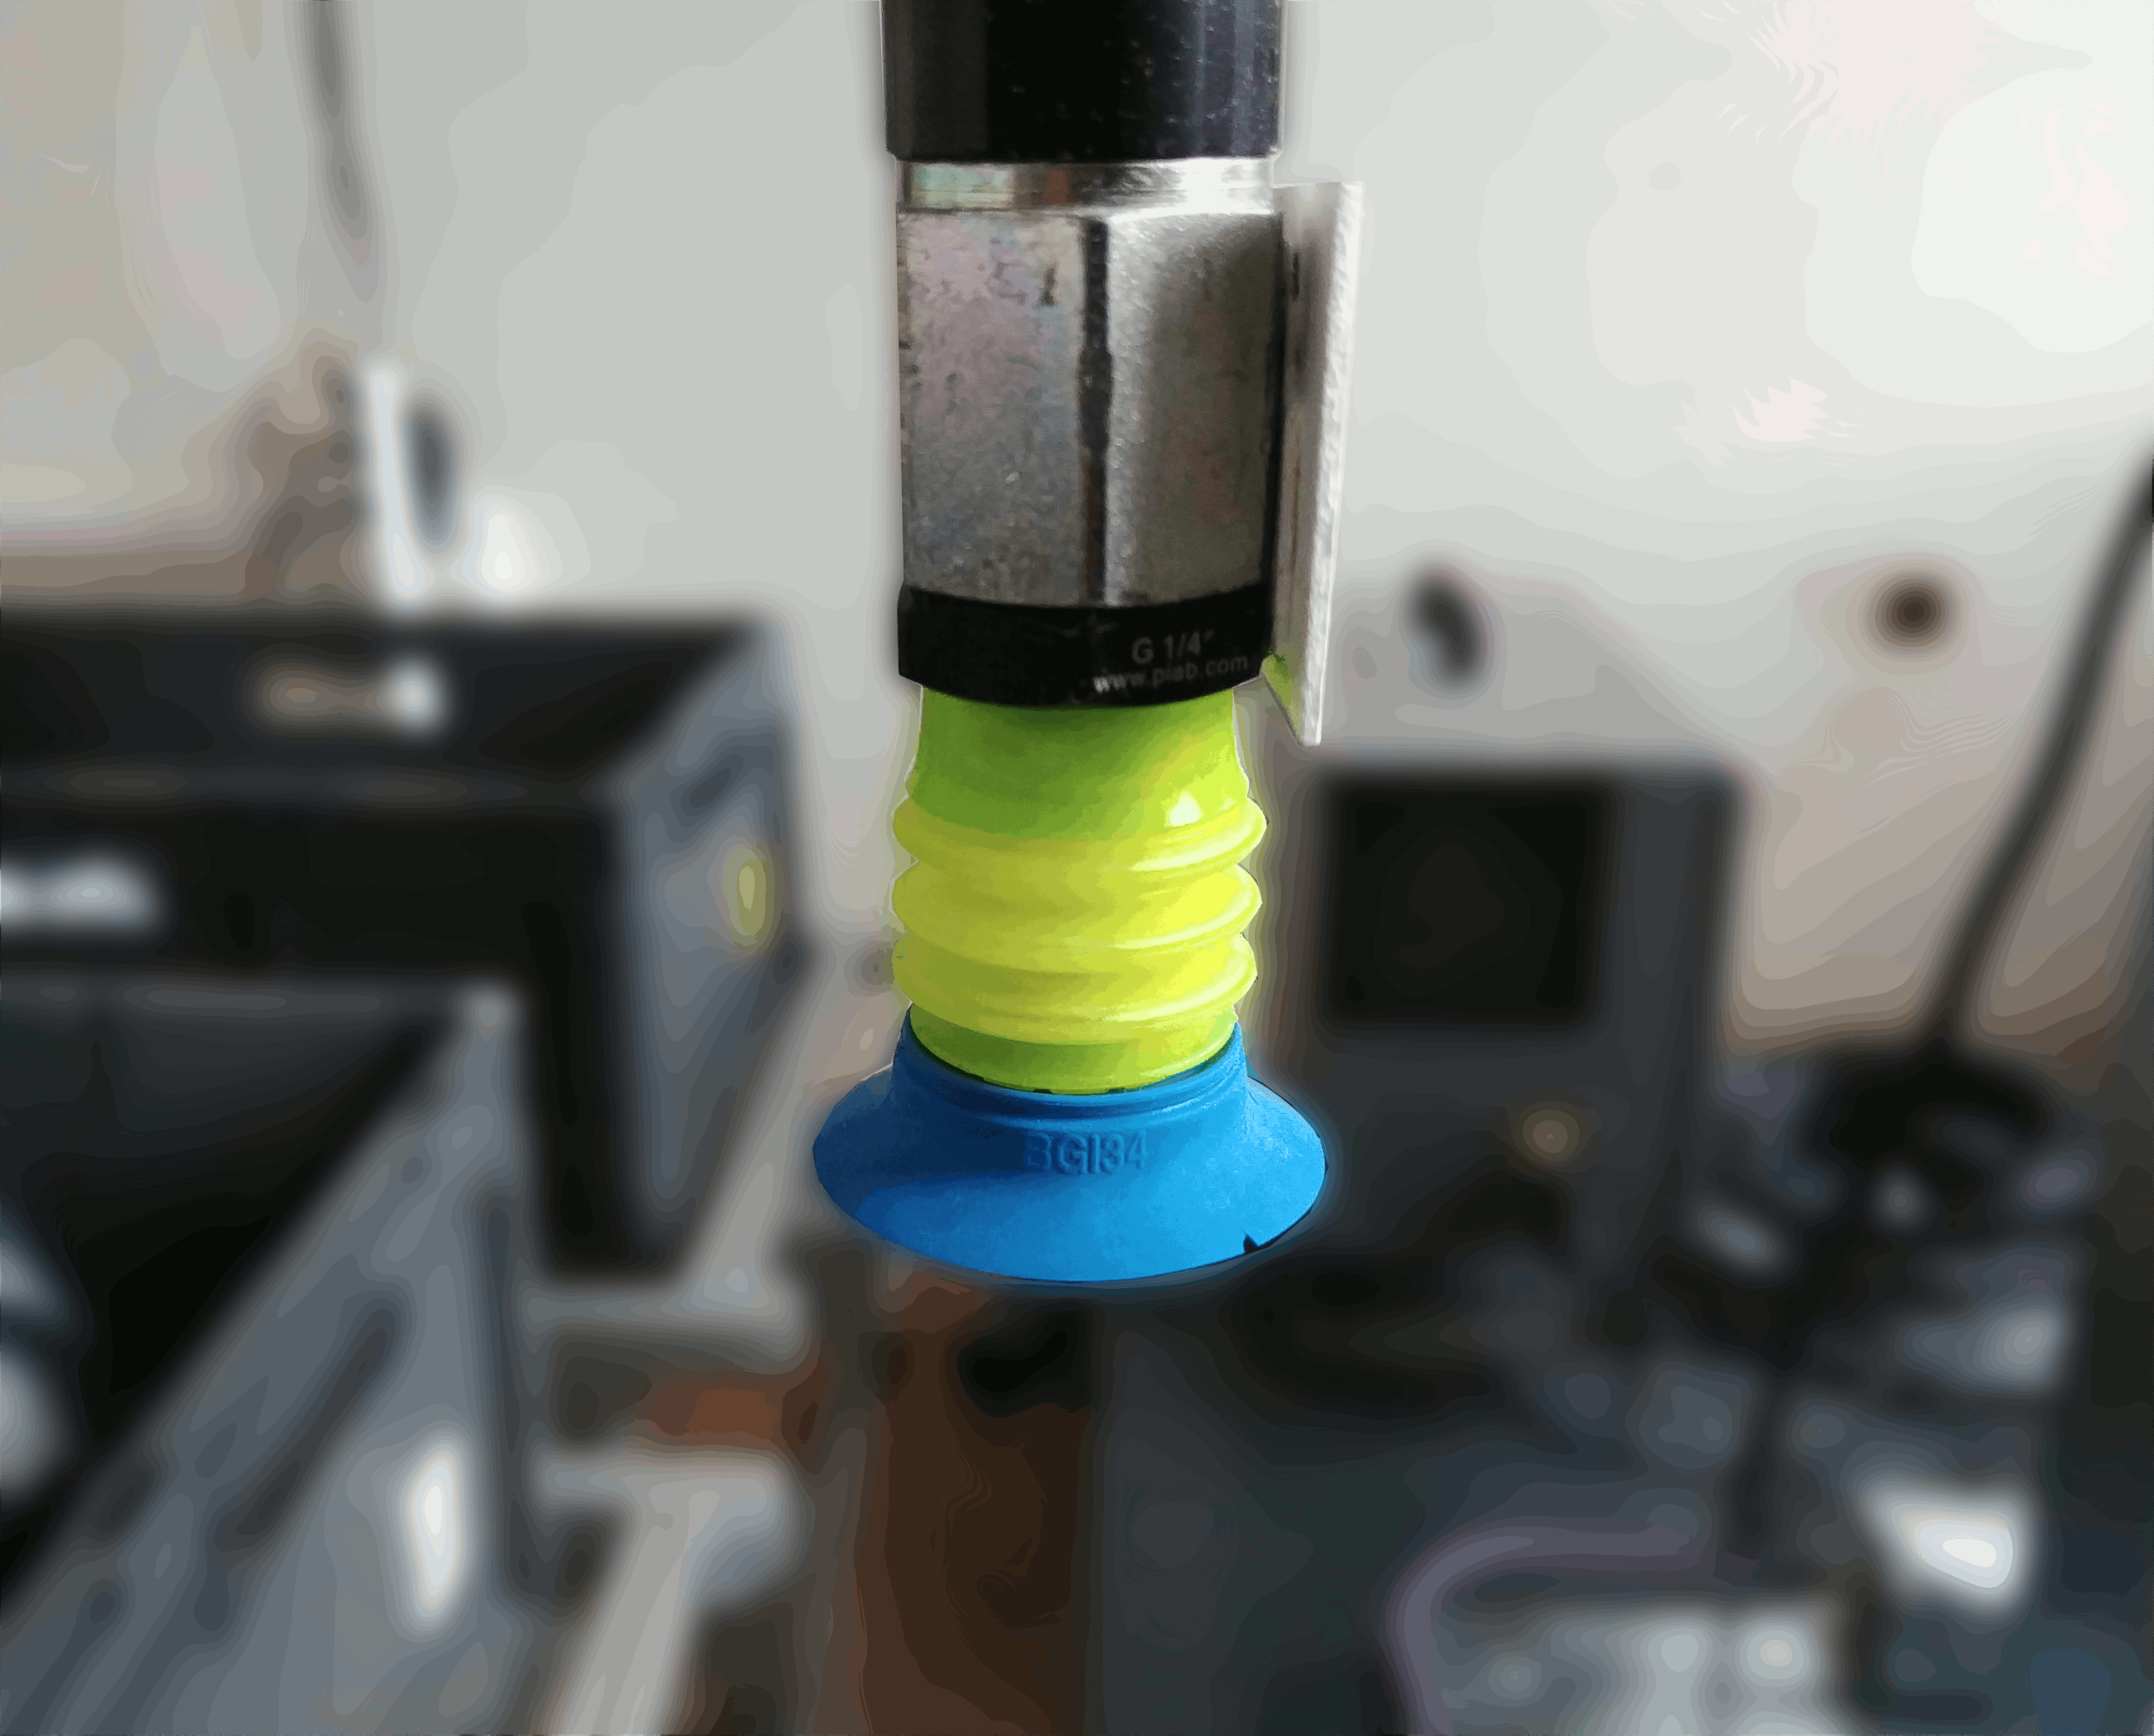
\includegraphics[scale=0.05]{\main/figures/suction_unloaded_indexed.png}
\caption{Unloaded}
\label{fig:background:suction-unloaded}
\end{subfigure}
\begin{subfigure}{0.49\textwidth}
\centering
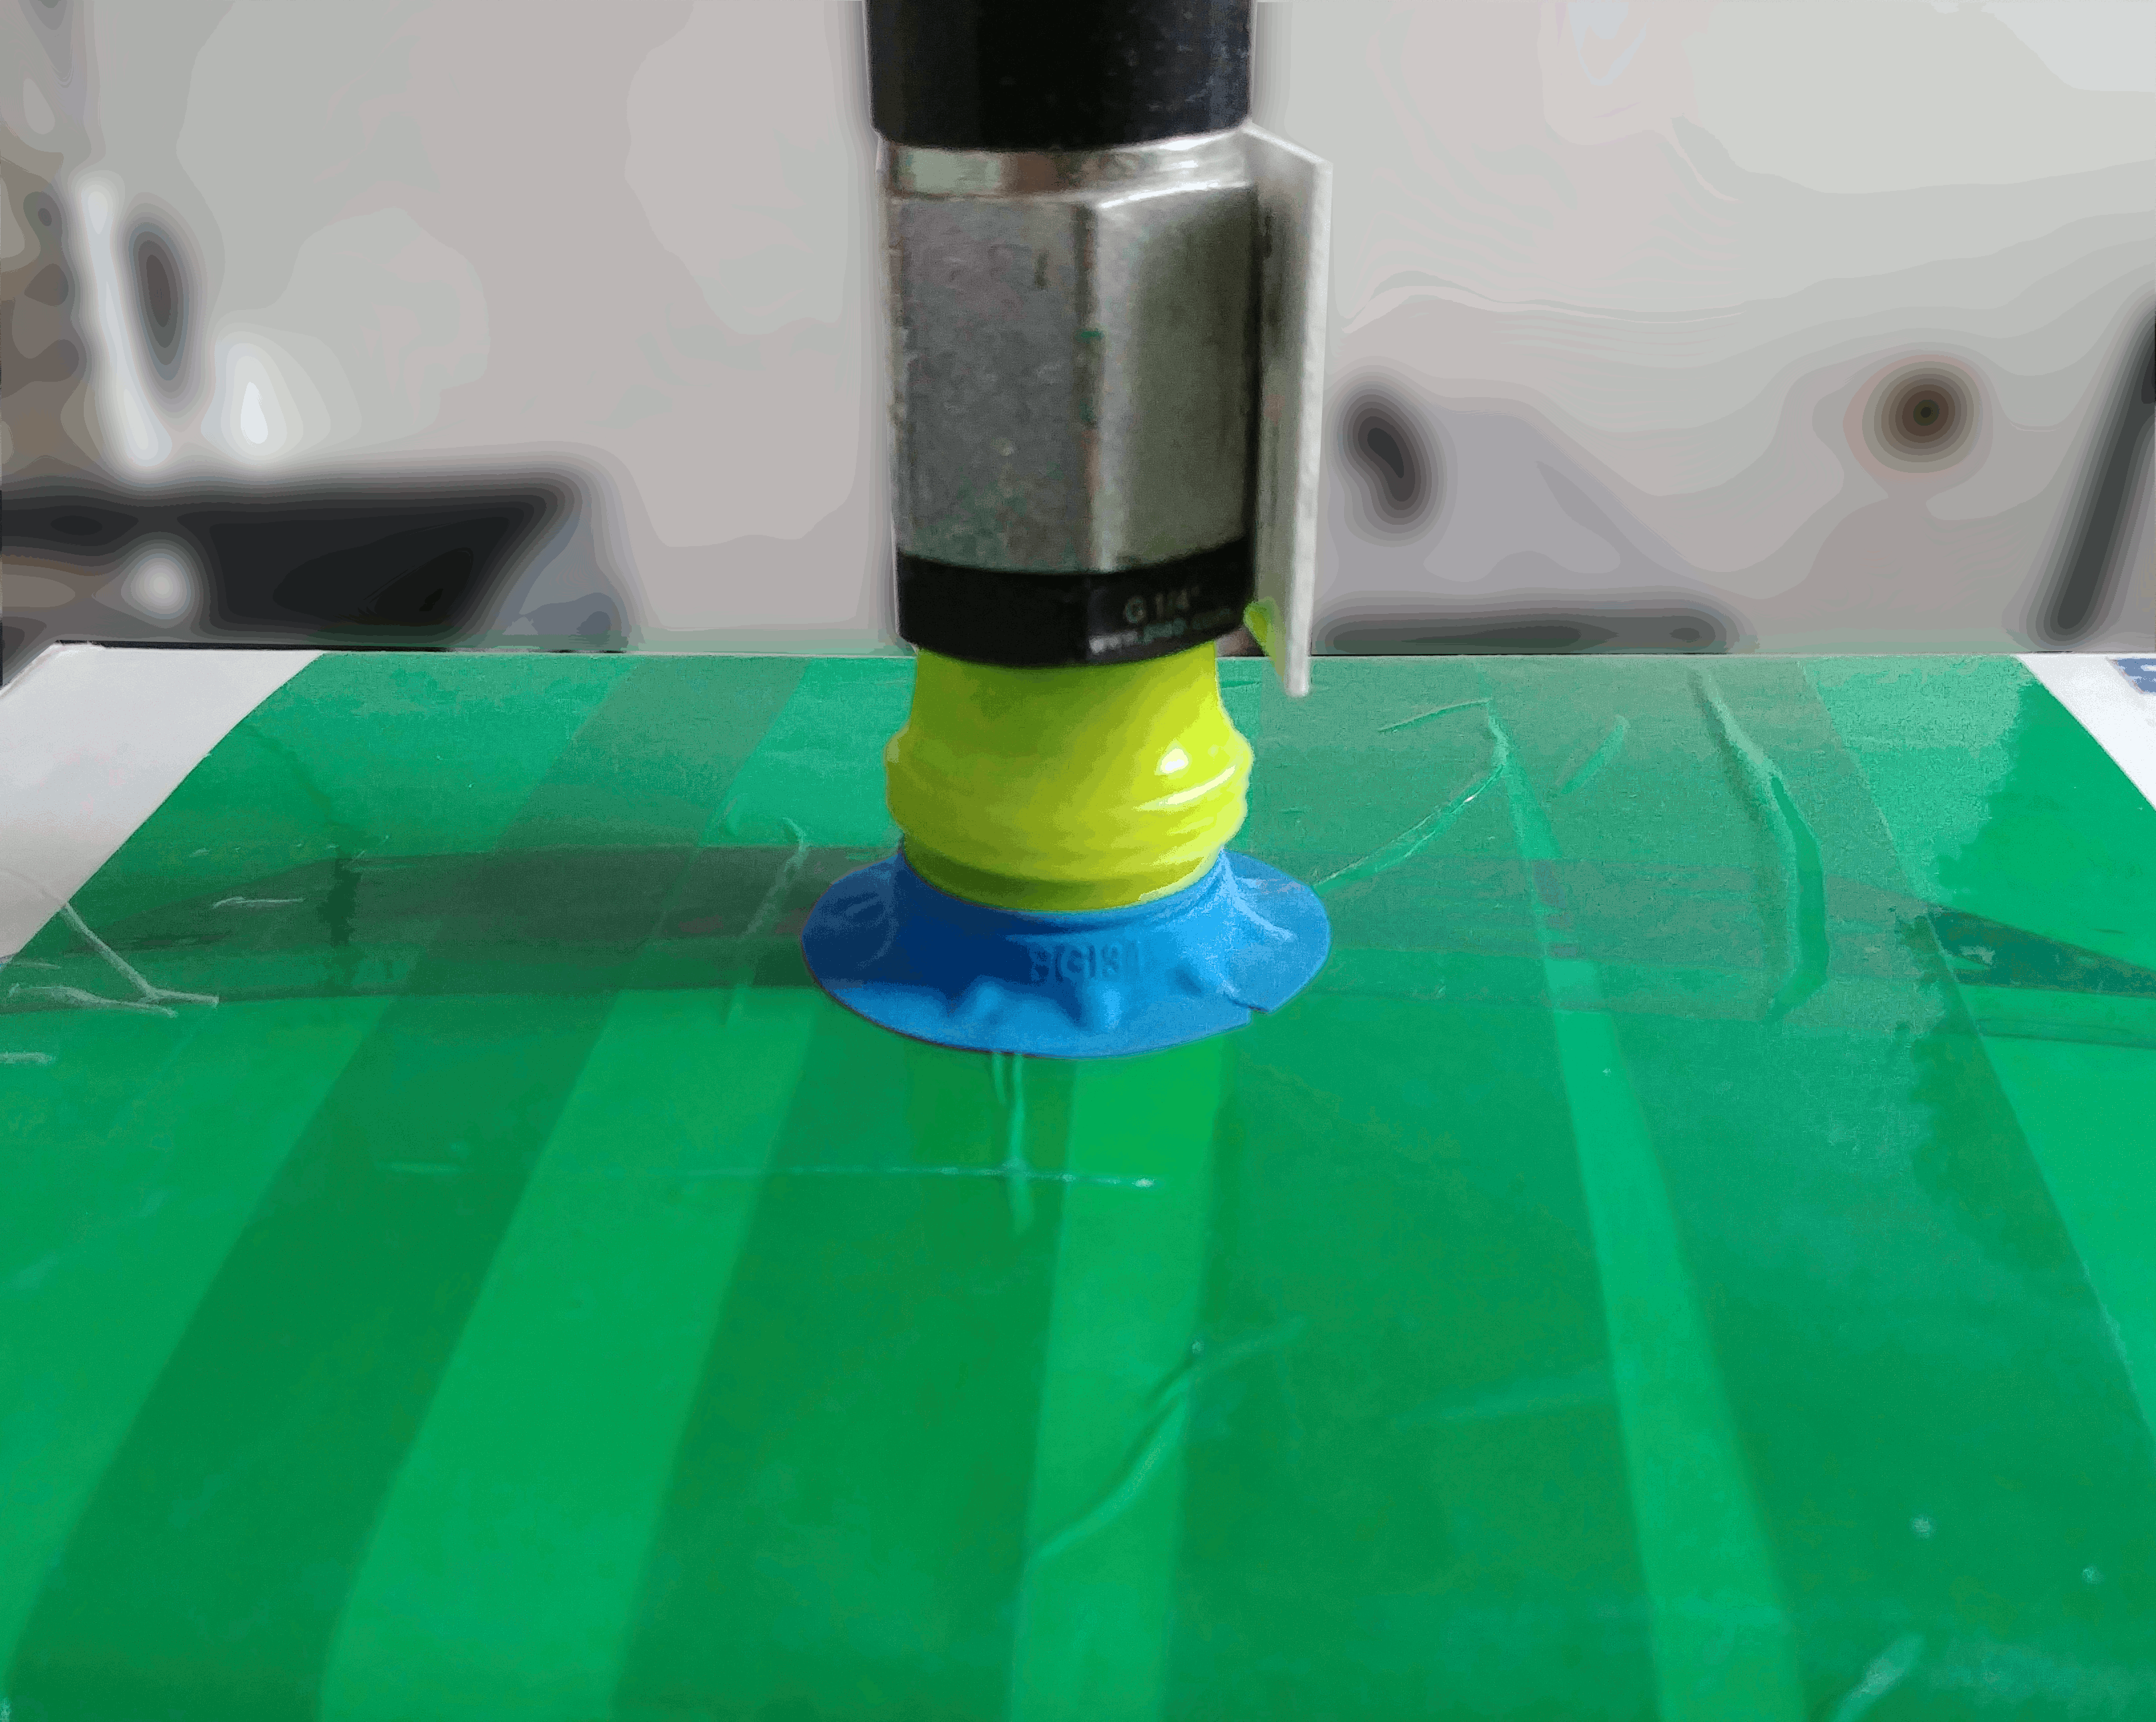
\includegraphics[scale=0.06]{\main/figures/suction_loaded_indexed.png}
\caption{Loaded}
\label{fig:background:suction-loaded}
\end{subfigure}
\caption{Vaccum suction cup gripper. The yellow part can twist with its srping shape in order to grasp tilted item. When a item is handled, the suction gripper is compressed by the air pressure. Note that the Tool Center Point (TCP) position is computed as the position of the extremity of the cup when it is not compressed. Images from the author.}
\label{fig:background:suction}
\end{figure}

\subsection{Characteristics of a typical \textit{pick-and-place} motion}
\label{background:motion}

In the context of \textit{pick-and-place} tasks, a robotic manipulator is meant to
take an item from a given initial pose to a final pose \cite{Angeles2006}. This type of operation is exploited in tasks like loading and unloading of conveyor belts, totes, carts. In the use case of the project, trajectories have a blending trapezoidal shape. They are optimized for high production cadence and grasping failure avoidance (cf. Figure \ref{fig:background:tote_cycle}).

\begin{figure}[h]
  \centering
  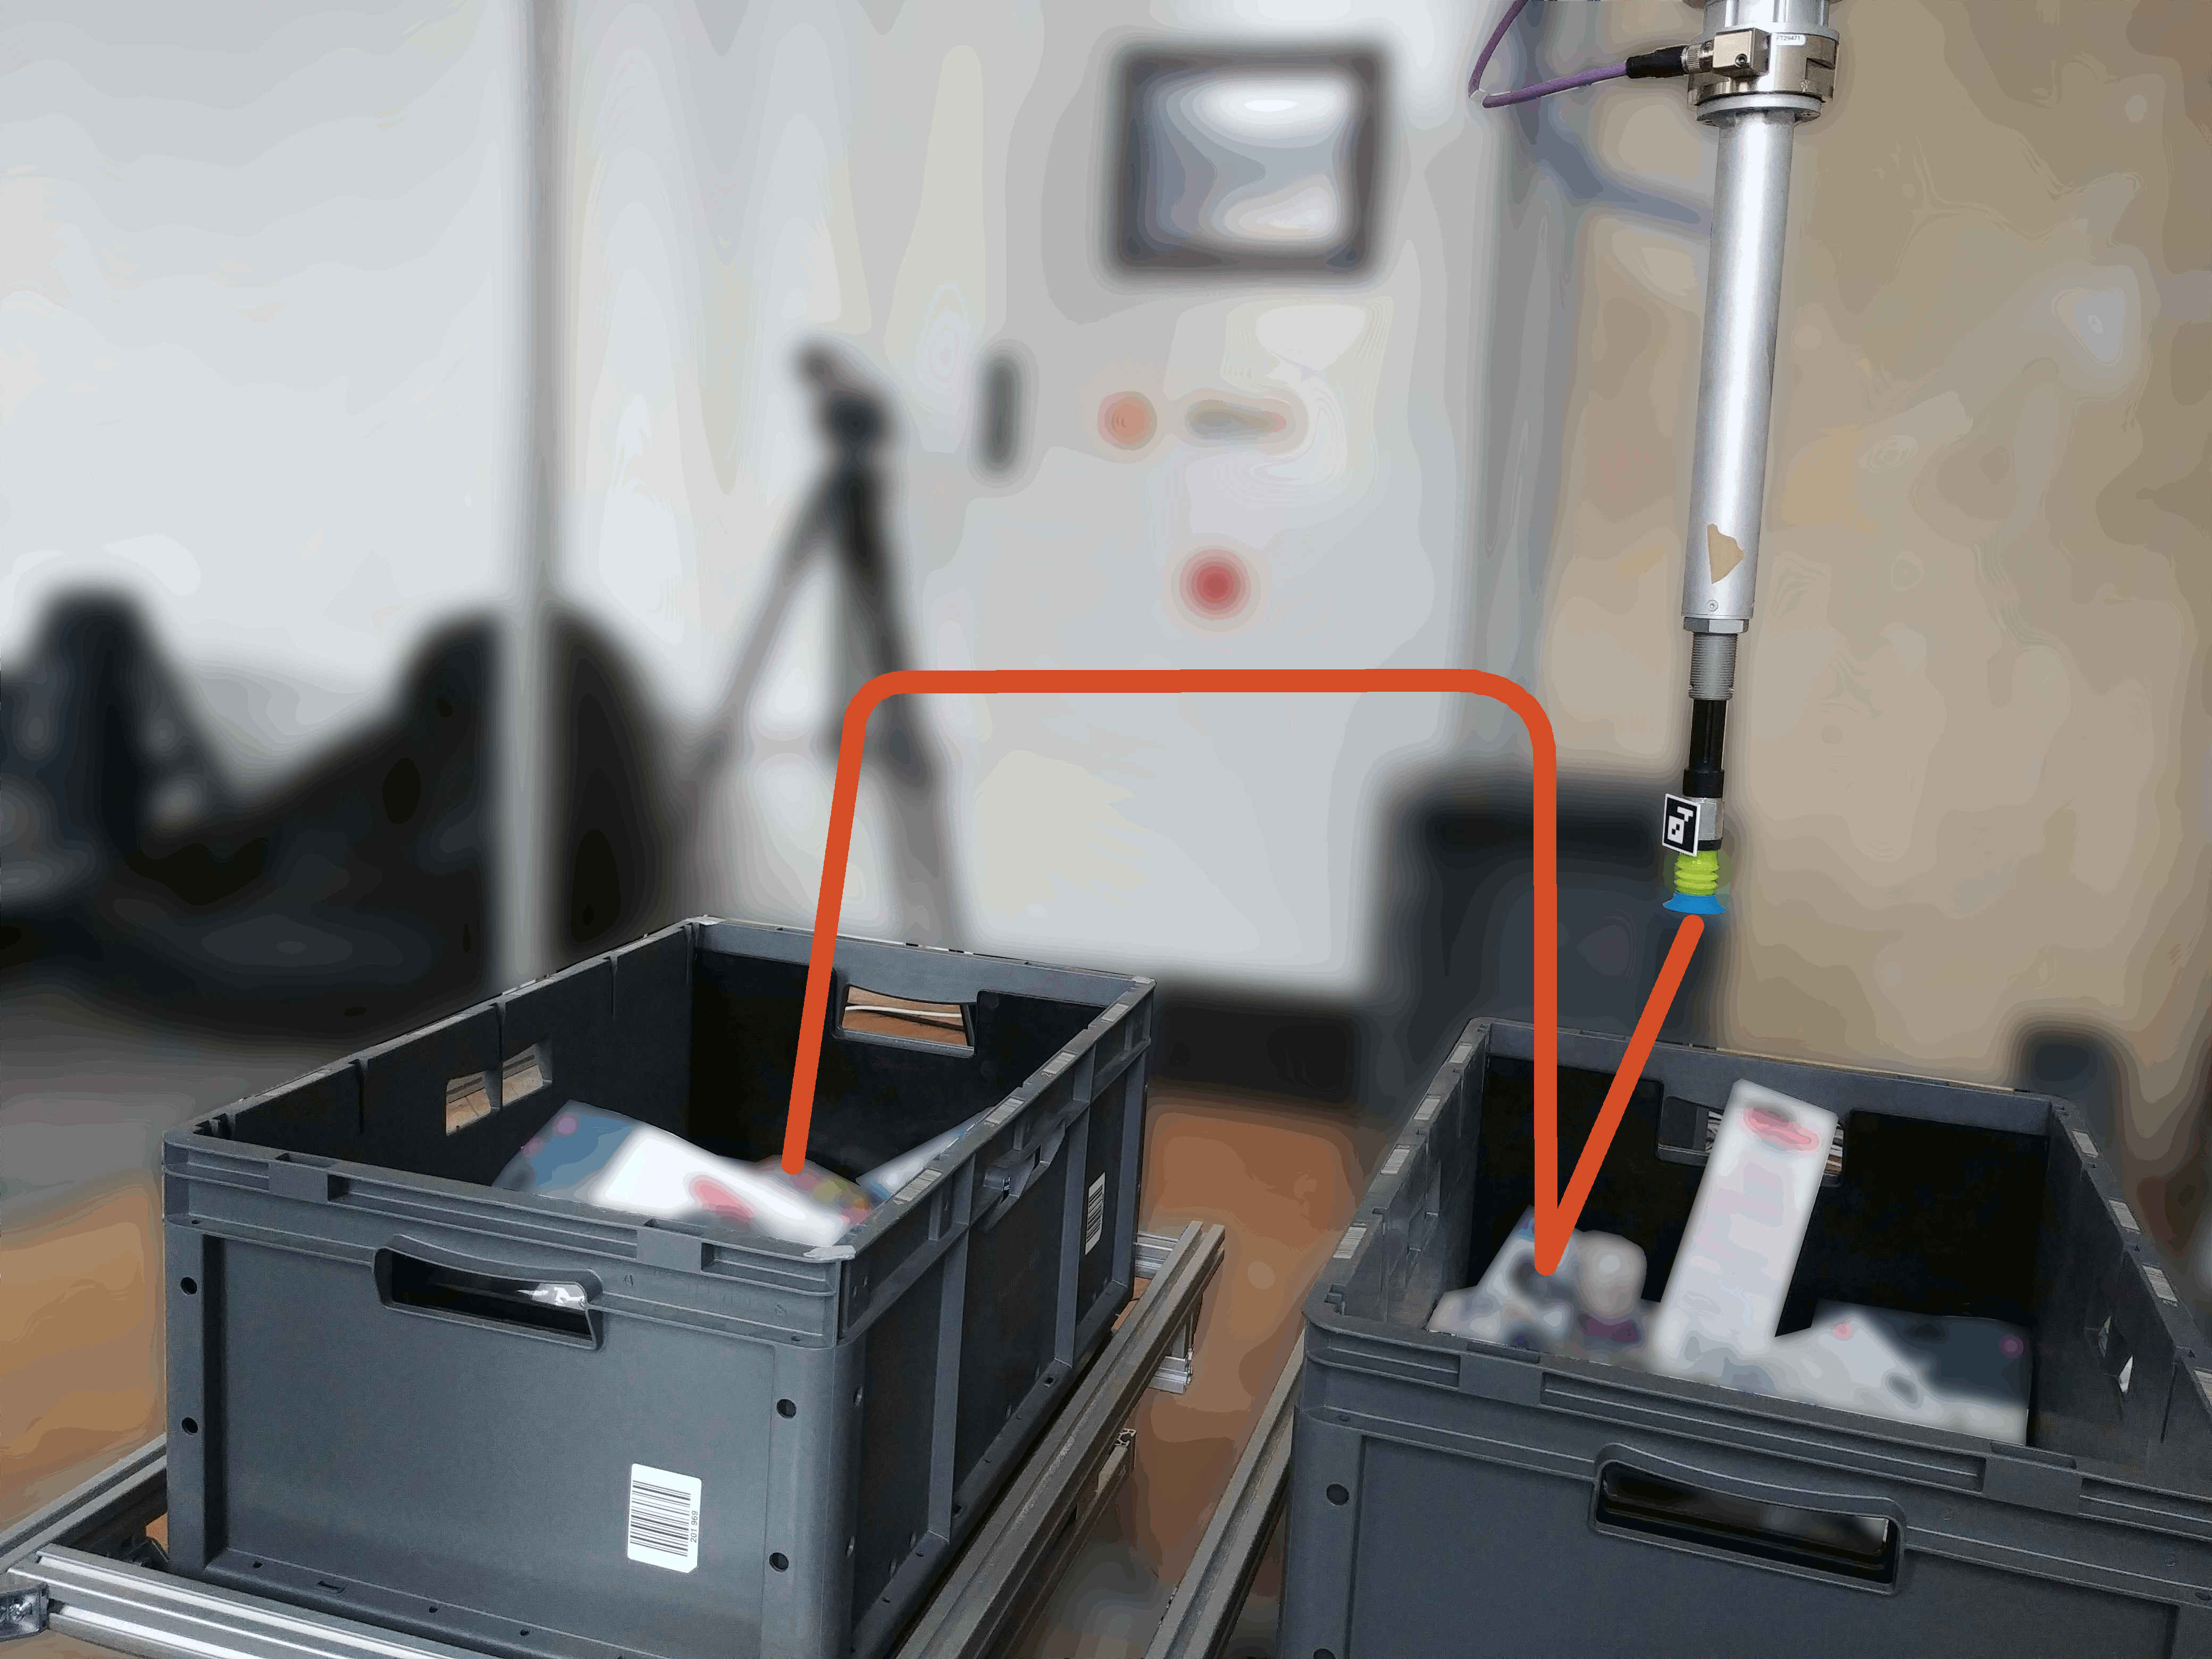
\includegraphics[scale=0.08]{\main/figures/tote_cycle_indexed.png}
  \caption{Trajectory of the Tool Center Point (TCP) during a \textit{pick-and-place} cycle. The tool goes in the tote until the contact with the item to grasped is made. Then it goes vertically up until it reaches a safety position where the item cannot hit the side of the tote or other items. Then the tool moves in the direction of the target tote to drop the item. The descent is slightly oblique to reduce jerk and optimize regarding the time. When it changes direction, the trajectory is blended for the same reasons.}
  \label{fig:background:tote_cycle}
\end{figure}

The drawback of using a suction cup for grasping is that the mechanical link between the tool and the item is not rigid. Heavy items and objects with large dimensions are very likely to oscillate during the motion. In logistic warehouses, robots often handle objects over half a kilo and longer dimension over $0.3 \si{\meter}$. Observations show that the angle between the tool and the item may vary significantly (up to $10 \si{\degree}$). Wobbling has a knock-on effect on \ac{FT} measurements. While there should not be any oscillations of the torque in a rigid model (for more detail, please refer to Section \ref{section:mechanical-models}), significant variations can be seen in actual measurement (cf. torque signal in the results section:   Figure \ref{fig:results:calibration:suction-torque-x}).

When it comes to physically modelling the system, different level of details can be taken into account. The first approach is to consider a rigid link between the tool and the item. The second approach is to fit an appropriate mechanical model considering the number of \ac{DoF} and the damped harmonic oscillator theory.

\section{Mechanical models}
\label{section:mechanical-models}

A lot of effort has been put into estimating the dynamic parameters of each rigid body link of robotic manipulators during the late century. An \textit{et al.} \cite{An1985} have developed a method to estimate the mass, the location of the center of mass and the moment of inertia of every link of a robotic arm. The method uses the joint torques and the calculation of the kinematics of the manipulator while moving. This work provides a sound method to derive the dynamic equations. Liu \textit{et al.} enhanced this approach in 1998 \cite{Liu1998} by using a proper filtering method for velocity that avoids difficult-to-measure acceleration measurements. Both teams were working with robotic manipulators mounted \textit{on} a six-axis \ac{FT} sensor screwed on a stand. The configuration is different in this project as the sensor is mounted on the last wrist. It is therefore easier to access the mass of payload as none of the joints as to be considered.

Nowadays, more compact \ac{FT} sensors are developed. Also, more complex use cases require to quantify robot interactions with its environment. Therefore, it is possible to mount \ac{FT} sensors on the last wrist and benefit from a more sensitive measurement. Several research projects have taken advantage of that and have developed payload inertial parameters estimation methods \cite{Kubus2008, Kubus2007, Kubus2014, Farsoni2018}. These methods similarly derive \textsc{Newton-Euler} equations to isolate a set of 10 inertial parameters: the mass, the center of mass and the independent inertia tensor coefficients.

This section presents the rigid-assumptions mechanical model and an observation-based Rotational Mass Spring Damper (RMSD) two-body model.

\subsection{Rigid model of the \{tool + item\} system}
\label{section:background:rigid}

The equations exploited to estimate the inertial parameters of the \{tool + item\} body (mass $m$, coordinates of the center of mass $c$, and inertia matrix $I$) are derived from the basic laws of dynamics. The motion of a rigid body (\{tool + item\}) due to external forces and torques can be described based on the \textsc{Newton-Euler} equations.

The assumptions are as followed (illustrated in Figure \ref{fig:tikz:one_body}):

\begin{itemize}
 \item \ac{FT} sensor ($S$) measures the force $f$ and torque $\tau$ applied on the \{tool + item\} system,
 \item the Tool Center Point (TCP) ($A$) moves with a linear acceleration $a$, an angular acceleration $\alpha$ and an angular velocity $\omega$,
 \item the \{tool + item\} system is composed of the extension tube, spring, suction cup –of total mass $m_1$, center of mass $c_1$ and inertia matrix $I_1$– and the object –of mass $m_2$, center of mass $c_2$ and inertia matrix $I_2$,
 \item centers of mass and inertia matrices are defined w.r.t.\ point $S$ such that $c = \overrightarrow{SG}$, $c_1 = \overrightarrow{SG_1}$ and $c_2 = \overrightarrow{SG_2}$.
\end{itemize}

\begin{figure}[h]
\centering
   % \documentclass[tikz]{standalone}

% \usetikzlibrary{patterns}

\tikzset{cross/.style={cross out, draw=black, minimum size=2*(#1-\pgflinewidth), inner sep=0pt, outer sep=0pt},
%default radius will be 1pt.
cross/.default={4pt}}


% \begin{document}
\begin{tikzpicture}[thick,>=latex,->]


\begin{scope}
\clip(-5,6) rectangle (5,-4);
% \draw[step=1cm,gray,very thin] (-5,6) grid (10,-5);

% \filldraw[white] (-4.3,4.3) rectangle (4.3,0);
% \draw[double distance=1.6mm] (0,0) -- (3,-3) node[midway,xshift=4mm,yshift=2mm]{$\ell$};
% \draw[->] (3,-3) -- (3,-4.5) node[below]{$m\cdot g$};
% \draw[->] (3,-3) -- (2.,-2.0) node[left,yshift=-3mm]{$F$};
% \draw[fill=white] (-.5,.25) -- (.5,.35) -- (1.2,0.2) -- (-1.2,-0.2) -- cycle;
% \draw[fill=white] (-.4,1) -- (-.7,.9) -- (-.3,.8) -- (-.7,.7) -- (-.3,.5) -- (-.7,.4) -- (-.5,.25) -- (.5,.35) --  (.7,.5) -- (.3,.6) -- (.7,.7) -- (.3,.8) -- (.7,.9) -- (.4,1) -- cycle;
\draw[fill=white] (-4, -3) -- (-4, 0) -- (4, 0) -- (4,-3) -- cycle;


% \draw[draw=black,fill=white] (0, 0) circle circle (.3cm);
% \draw[draw=black,fill=white] (3,-3) circle circle (.3cm);
\draw[->] (2.6,4.1) -- (4,4.1) node[above]{$\overrightarrow{y_0}$};
\draw[->] (2.6,4.1) -- (2.6,5.5) node[right]{$\overrightarrow{z_0}$};

% \draw[dash dot] (0,0) -- (2.55,0) node[below]{$\overrightarrow{y_0}$};
% \draw[dash dot] (0,0) -- (2.5, .42) node[above]{$\overrightarrow{y_2}$};
% \draw[thick] ([shift=(0:2cm)]0,0) arc (0:20:1cm);
% \node[] at (2.3, .2) {$\theta$};

\draw[pattern=north east lines] (-.4,5.5) rectangle (.4,0);

\node[right] at (.5,5.5) {$S(y_1, z_1)$};
\draw[fill=white] (-.1, 5.4) -- (.1, 5.6) -- cycle;
\draw[fill=white] (-.1, 5.6) -- (.1, 5.4) -- cycle;

\node[below right] at (0,0) {A};
\draw[fill=white] (-.1, -.1) -- (.1, .1) -- cycle;
\draw[fill=white] (-.1, .1) -- (.1, -.1) -- cycle;

\node[right] at (0.3,1.5) {$G$};
\draw[fill=white] (-.1, 1.4) -- (.1, 1.6) -- cycle;
\draw[fill=white] (-.1, 1.6) -- (.1, 1.4) -- cycle;

\node[right] at (.2,-1.5) {$G_2$};
\draw[fill=white] (-.1, -1.6) -- (.1, -1.4) -- cycle;
\draw[fill=white] (-.1, -1.4) -- (.1, -1.6) -- cycle;

\node[right] at (0.3,2.5) {$G_1$};
\draw[fill=white] (-.1, 2.4) -- (.1, 2.6) -- cycle;
\draw[fill=white] (-.1, 2.6) -- (.1, 2.4) -- cycle;

\node[rotate=0] at (-3,-0.5) {$m_2$, $I_{2,A}$};

\end{scope}

\end{tikzpicture}
% \end{document}
 %     without .tex extension
   % or use \input{mytikz}
   \caption{Schematic diagram of the \{tool + item\} rigid system. \{0\} characterizes the base frame, \{1\} the tool and \{2\} the item.}
   \label{fig:tikz:one_body}
\end{figure}

\subsubsection{Formulation of the \textsc{Newton-Euler} equations}
\label{subsubsection:background_newton_equation}

Detailed derivation of the \textsc{Newton-Euler} equation is presented in Appendix \ref{appendix:models}. The method followed is fairly similar to the one proposed in \cite{An1985} except that equations are directly determined w.r.t.\ point $A$, in the base link frame. This variation paves the way to the second model which is derived in a similar fashion.

The dynamics of the rigid body is described by the equations \ref{background:eq:rigid} (and equations \ref{appendix:eq:rigid} in Appendix \ref{appendix:models}), also used in \cite{Kubus2008, Kubus2007, Kubus2014, Farsoni2018}. They are \textit{linear} w.r.t.\ to the unknown parameters.

\begin{equation}
 \label{background:eq:rigid}
 \left \{
 \begin{array}{l l}
  f =    & m (a - g) + \omega \times (\omega \times m c) + \alpha \times m c \\
  \tau = & m c \times (a - g)
  + I_{S} \ast \alpha + \omega \times (I_{S} \ast \omega)
 \end{array}
 \right.
\end{equation}

where $I_S = I_S^T =
\begin{pmatrix}
 I_{xx} & I_{xy} & I_{xz} \\
 I_{xy} & I_{yy} & I_{yz} \\
 I_{xz} & I_{yz} & I_{zz}
\end{pmatrix}
$.

The equation \ref{background:eq:rigid} is exploited to compose the matrix equation \ref{background:eq:inertia_estimation} (cf. Section \ref{appendix:rigid:inertia_estimation} for detailed expression). This equation allows to isolate the 10 inertial parameters to be estimated. It can be easily adapted for least-squares-based estimation methods.

\begin{equation}
  \label{background:eq:inertia_estimation}
B = A(a, \alpha, \omega, g) \varphi
\end{equation}

where $B =  \begin{pmatrix} f \\ \tau \end{pmatrix}$ and $\varphi = [m, m c_x, m c_y, m c_z, I_{xx}, I_{xy}, I_{xz}, I_{yy}, I_{yz}, I_{zz}]^T$ contains the 10 independant inertial parameters and $A$ is defined in section \ref{appendix:rigid:inertia_estimation}.

Linearity w.r.t.\ $\varphi$ gives the opportunity to easily subtract the tool inertial parameters $\varphi_1$ to the \{tool + item\} system to get the item inertial parameters $\varphi_2$ (cf. equation \ref{eq:background:rigid:phi}). One can note that the center of mass of multiple corpses is by definition: $c = \frac{m_1 c_1 + m_2 c_2}{m_1 + m_2}$. It further confirms that $mc = m_1 c_1 + m_2 c_2$.

\begin{equation}
  \label{eq:background:rigid:phi}
  \varphi_2 = \varphi - \varphi_{1}
\end{equation}


\subsection{Rotational Mass Spring Damper model of the \{tool + item\} system}
\label{section:background:rmsd}

As mentioned in section \ref{background:motion}, the elasticity of the suction cup generate oscillations of the item w.r.t.\ the tool that are not taken into account by the one-rigid-body model. The object rotates in fact about the $x_1$-axis and the $y_1$-axis. There is no translation motion w.r.t.\ the tool and no rotation about the $z_0$-axis. Therefore, the mechanical link between the item and the tool can be identified as a \ac{UJ} –as known as \textsc{Cardan} joint (cf. Figure \ref{fig:background:cardan}). With this mechanical connection, the tool can only transfer forces, and torque about the lengthwise axis of the sensor but no torque about the transversal axes.

\begin{figure}[h]
  \centering
  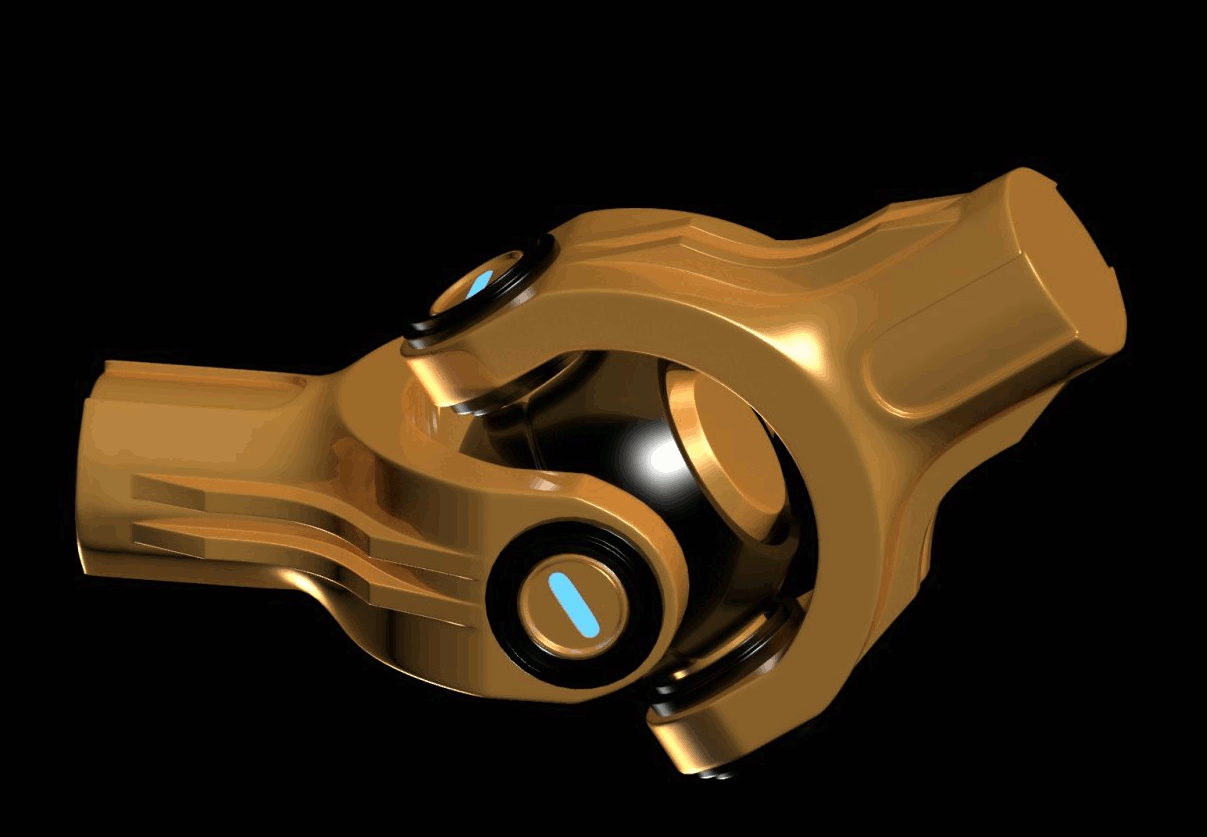
\includegraphics[scale=0.3]{\main/figures/cardan_joint_indexed.png}
  \caption{3D model of a 2 \ac{DoF} \ac{UJ}. Image from \cite{3dexport2020}.}
  \label{fig:background:cardan}
\end{figure}

One can notice that the combination of the two bodies behaves as a 2 \ac{DoF} harmonic pendulum. Thus, the torque transmitted by the tool \{1\} to the item \{2\} about the $x$-axis –or $y$-axis– is modeled by $T_{1/2, x} = k_x \theta_{1/2, x} + \lambda_x \dot{\theta}_{1/2, x}$ with $k_x$ a spring constant,  $\lambda_x$ a damping coefficient and $\theta_{1/2, x}$ the orientation of the tool w.r.t.\ the item about the $x$-axis (Figure \ref{fig:tikz:two_bodies}). In addition, the suction cup is symetrical by rotation about the lengthwise axis of the tool. For this reason, it is considered that $k_x = k_y = k$ and $\lambda_x = \lambda_y - \lambda$. Also, in the specific case of \textit{pick-and-place} tasks, it can be considered that the inertia parameters estimation is processed while the tool is vertical. That simplifies equations by infering that $\overrightarrow{z_1} = -\overrightarrow{z_0}$.

\begin{figure}[h]
\centering
   % \documentclass[tikz]{standalone}

% \usetikzlibrary{patterns}

\tikzset{cross/.style={cross out, draw=black, minimum size=2*(#1-\pgflinewidth), inner sep=0pt, outer sep=0pt},
%default radius will be 1pt.
cross/.default={4pt}}


% \begin{document}
\begin{tikzpicture}[thick,>=latex,->]


\begin{scope}
\clip(-5,6) rectangle (5,-4);
% \draw[step=1cm,gray,very thin] (-5,6) grid (10,-5);

% \filldraw[white] (-4.3,4.3) rectangle (4.3,0);
% \draw[double distance=1.6mm] (0,0) -- (3,-3) node[midway,xshift=4mm,yshift=2mm]{$\ell$};
% \draw[->] (3,-3) -- (3,-4.5) node[below]{$m\cdot g$};
% \draw[->] (3,-3) -- (2.,-2.0) node[left,yshift=-3mm]{$F$};
\draw[fill=white] (-.5,.25) -- (.5,.35) -- (1.2,0.2) -- (-1.2,-0.2) -- cycle;
\draw[fill=white] (-.4,1) -- (-.7,.9) -- (-.3,.8) -- (-.7,.7) -- (-.3,.5) -- (-.7,.4) -- (-.5,.25) -- (.5,.35) --  (.7,.5) -- (.3,.6) -- (.7,.7) -- (.3,.8) -- (.7,.9) -- (.4,1) -- cycle;
\draw[fill=white] (-3.5, -3.6) -- (-4,-.667) -- (4,.667) -- (4.5,-2.27) -- cycle;


% \draw[draw=black,fill=white] (0, 0) circle circle (.3cm);
% \draw[draw=black,fill=white] (3,-3) circle circle (.3cm);
\draw[->] (2.6,4.1) -- (4,4.1) node[above]{$\overrightarrow{y_0}$};
\draw[->] (2.6,4.1) -- (2.6,5.5) node[right]{$\overrightarrow{z_0}$};

\draw[->] (0.0,5.5) -- (-1.4,5.5) node[below]{$\overrightarrow{y_1}$};
\draw[->] (0.0,5.5) -- (0.0,4.1);
\node[left] at (-0.3,4.1) {$\overrightarrow{z_1}$};


\draw[dash dot] (0,0) -- (2.55,0) node[below]{$\overrightarrow{y_0}$};
\draw[dash dot] (0,0) -- (-2.5, -.42) node[above]{$\overrightarrow{y_2}$};
\draw[thick] ([shift=(0:2cm)]0,0) arc (0:20:1cm);
\node[] at (2.3, .2) {$\theta$};

\draw[pattern=north east lines] (-.4,5.5) rectangle (.4,1);

\node[right] at (.5,5.5) {$S(y_1, z_1)$};
\draw[fill=white] (-.1, 5.4) -- (.1, 5.6) -- cycle;
\draw[fill=white] (-.1, 5.6) -- (.1, 5.4) -- cycle;

\node[below right] at (0,0) {A};
\draw[fill=white] (-.1, -.1) -- (.1, .1) -- cycle;
\draw[fill=white] (-.1, .1) -- (.1, -.1) -- cycle;

\node[right] at (0.3,1.5) {$G$};
\draw[fill=white] (.0, 1.4) -- (.2, 1.6) -- cycle;
\draw[fill=white] (.0, 1.6) -- (.2, 1.4) -- cycle;

\node[right] at (0.25,-1.46) {$G_2$};
\draw[fill=white] (.15, -1.56) -- (.35,-1.36) -- cycle;
\draw[fill=white] (.15, -1.36) -- (.35, -1.56) -- cycle;

\node[right] at (0.3,2.5) {$G_1$};
\draw[fill=white] (-.1, 2.4) -- (.1, 2.6) -- cycle;
\draw[fill=white] (-.1, 2.6) -- (.1, 2.4) -- cycle;

\node[rotate=10] at (-3,-0.8) {$m$, $I_{2,A}$};

\end{scope}

\end{tikzpicture}
% \end{document}
 %     without .tex extension
   % or use \input{mytikz}
   \caption{\ac{RMSD} \{tool\} and \{item\} system.}
   \label{fig:tikz:two_bodies}
\end{figure}

This said, the total mechanical action on the item \{2\} by the tool \{1\} is as follows (cf. \ref{appendix:notation:wrench} for notation):

{\centering
 $ \{ \mathcal{V}_{1/2} \}
 = \leftidx{_{A}}{
  \left \{ \begin{array}{c}
  \overrightarrow{F}_{1/2} \\
  -N_{2/1} \overrightarrow{z_1} +  K \ast \overrightarrow{\Theta}_{1/2} + \Lambda \ast \overrightarrow{\Omega}_{1/2}
  \end{array} \right \}
  }{}
 $
 \par}

 with $\overrightarrow{\Theta}_{1/2}$ the orientation of \{1\} w.r.t.\ \{2\}, $\overrightarrow{\Omega}_{1/2}$ the angular speed of \{1\} w.r.t.\ \{2\} and $K = diag(k, k, 0)$ and $\Lambda = diag(\lambda, \lambda, 0)$.

 By isolating the tool \{1\} only and then applying the \ac{FPD} (cf. equation \ref{appendix:notation:fpd}) to this system, the tool/item orientation $\overrightarrow{\Theta}_{1/2}$ and angular speed $\overrightarrow{\Omega}_{1/2}$ can be derived as function of the torque $\tau$ and of the inertial parameters of the tool $\varphi_1$ (cf. section \ref{appendix:rmsd:fpd1}).

 In a similar way to previous section (cf. \ref{section:background:rigid}), the relation between the kinetic measurements and the inertial parameters of the item $\varphi_2$ can be derived as a matrix equation (cf. equation \ref{eq:background:rmsd_inertia_estimation}).

 \begin{equation}
   \label{eq:background:rmsd_inertia_estimation}
 B' = A'(a, \alpha_1, \alpha_2, \omega_1, \omega_2, \theta_2, g) \varphi_2
 \end{equation}

 where  $B' = \begin{pmatrix} f' \\ \tau' \end{pmatrix}$, $\varphi_2$ contains the 10 independant inertial parameters of the item, $A'$, $f'$ and $\tau'$ are defined in the appendix \ref{appendix:msd:inertia_estimation}.

Now that relation between the \ac{FT} measurement and the kinematics of the robot manipulator have been brought to life, a method to estimate the item inertial parameters has to be developed.

\section{Estimation Approaches}
\label{section:estimation}

In this section, a brief introduction to Least-Squares methods is presented followed by a focus on the Recursive Total Least-Squares (RTLS) approach.

Two physical models of the tool and item system have been developed in section \ref{section:mechanical-models}. Out of these two models, a linear matrix equation describing the dynamics of the assembly have been derived. These matrix equations are of the form: $B = A\varphi$. The objective consists of adjusting the parameters $\varphi$ of the model function $B = A\varphi$ to best fit the data set. The data set consists of $n$ pairs of matrices ($(B_i, A_i)_{i \in [1, n]}$) which are found by measuring the \ac{FT} and \ac{TCP} poses. The fit of the model to the data set is measured by its residual $r_i$, defined as the norm of the difference between the actual value of the dependent variable $B_i$ and the value predicted by the model $A_i \varphi$ \cite{Simoncelli2003}.

\subsection{Least-Squares method}
\label{subsection:ls}

The first approach considered is the \ac{LS} regression which is the most basic form of the \ac{LS} optimization problem. This problem has an innate connection to distances in Euclidean geometry. The aim is to find the set of parameters $\varphi$ that minimize the sum of the squared residuals:

\begin{equation}
  \argmin_{\varphi} \sum_{i=1}^{n} r_i^2 = \argmin_{\varphi} \sum_{i=1}^{n} ||B_i - A_i \varphi||^2
\end{equation}

To derive the sum, the strategy is to stack the $(B_i, A_i)_{i \in [1, n]}$ matrices over time. Here, $\Xi$ denotes a stack of matrices. In such way that $B_\Xi = [B_1^T, B_2^T, \ldots, B_n^T]^T$ and $A_\Xi = [A_1^T, A_2^T, \ldots, A_n^T]^T$. Then the optimisation problem can be simply written down as:

\begin{equation}
  \label{eq:background:stacked-ls}
  \min_{\varphi} ||B_\Xi - A_\Xi \varphi||^2
\end{equation}

There are potentially two options to compute the \ac{LS} curve fitting. The first one is to use a \ac{TRF} algorithm\footnote{This method is further implemented using the \textsc{Scipy} method \texttt{scipy.optimize.least\_squares}.}. The second is to use the \ac{SVD} of the $A$ matrix (cf. \cite{Gander2008}). The objective is to compute a pseudo-inverse of $A$ to be able to simply multiply it with $B$. The pseudo-inverse of a diagonal non-square matrix is a matrix with transposed dimensions and inverse values on the diagonal:

\begin{align*}
  \Sigma =
  \begin{pmatrix}
    a_1 & 0 & 0 & 0 \\
    0 & a_2 & 0 & 0 \\
    0 & 0 & a_3 & 0
  \end{pmatrix}
  &
  \ \Sigma^{-1} =
  \begin{pmatrix}
    \frac{1}{a_1} & 0 & 0 \\
    0 & \frac{1}{a_2} & 0 \\
    0 & 0 & \frac{1}{a_3} \\
    0 & 0 & 0
  \end{pmatrix}
\end{align*}


Algorithm \ref{alg:background:svd-ls} presents the method.

\begin{algorithm}
\caption{Estimate $\varphi$ with a \ac{SVD} \ac{LS} method \label{alg:background:svd-ls}}
\begin{algorithmic}
\STATE $U, \Sigma, V^T \leftarrow \text{\texttt{SVD}}(A)$
\STATE $\Sigma^{-1} \leftarrow \text{\texttt{pseudo\_inverse}}(\Sigma)$
\STATE $\varphi \leftarrow V \cdot \Sigma^{-1} \cdot U^T \cdot B$
\RETURN $\varphi$
\end{algorithmic}
\end{algorithm}

The \ac{LS} is the simplest solution to implement, yet, there is a drawback. The error model does not fit the framework of the situation. This method is indeed based on the assumption that the data matrices $A_i$ are free of errors. The error is simply modelled as a \ac{FT} error of measurement ($e_B$) such that: $\overline{B} = B + e_B$ with $\overline{B}$ the ground-truth value. This error model does not consider error in the data matrix $A(a, \alpha, \omega, g)$: $e_A$. Thus it does not consider the error in the gravity vector, \ac{TCP} pose measurements, and in the computation of the derivatives of the position and the orientation. Yet, the output signals presented in the results section \ref{section:results:pre-processing} clearly show noise and disturbances.

Besides, another disadvantage of this technique is that all computations have to be done offline. The approach is to collect the data during an adequate duration. Then, they have to be processed so that an estimated mass can be output. In the context of industrial robotics (cf. chapter \ref{chapter:introduction}), systems have to process data at a great speed and should be able to address hard failures as soon as possible. An ideal optimizer would be able to make an online estimation of the mass. It would recursively compute estimated masses with increasing precision as more data are gathered.

\subsection{Recursive Total Least-Squares method}

Intending to address the downsides of a simple \ac{LS} estimation, the \ac{RTLS} approach is introduced.

As stated above, the \ac{LS} method only assumes that the data matrix $B$ is a source of error and the data matrix $A$ is free of errors (cf. section \ref{subsection:ls}). Thereby, a method that takes into account errors in position, orientation, linear and angular speed, and linear and angular acceleration might perform better. The \ac{TLS} method explicitly take into consideration the error in the $A$ matrix (cf. equation \ref{eq:background:tls-error}) as explain by \textsc{Golub} \textit{et al.} \cite{Golub1980}. The figure illustrates the difference between the \ac{LS} and the \ac{TLS} approach \ref{fig:background:ls-tls-error}. The \ac{LS} method considers the error as the sum of the squared \textit{vertical} distances between the model and the data set whereas the \ac{TLS} considers the sum of the squared \textit{orthogonal} distances between the model and the data set. Hence, the \ac{TLS} algorithm takes into account disturbance and noise in \ac{FT} measurements \textit{as well as} the accelerations and angular velocities.

\begin{equation}
  \label{eq:background:tls-error}
B + e_B = (A + e_A) \varphi
\end{equation}

\begin{figure}[h]
\centering
\begin{subfigure}{0.49\textwidth}
\centering
\includegraphics[scale=1]{\main/figures/ls_comparison.pdf}
\caption{\ac{LS} error model}
\label{fig:background:ls-error}
\end{subfigure}
\begin{subfigure}{0.49\textwidth}
\centering
\includegraphics[scale=1]{\main/figures/tls_comparison.pdf}
\caption{\ac{TLS} error model}
\label{fig:background:tls-error}
\end{subfigure}
\caption{Data-fitting with the \ac{LS} and \ac{TLS} approches. The \ac{LS} method only consider error in the y-direction. \ac{TLS} also consider error in the x-direction.}
\label{fig:background:ls-tls-error}
\end{figure}

Besides, to provide an online estimation of the inertial parameters of the payload, it is required to recursively update the estimation. Using the \ac{TLS} algorithm in a recursive fashion seems tedious as it required to update the \ac{SVD} at each estimation cycle. Therefore, it is necessary to provide an efficient method to update the \ac{SVD}. For that reason, the \ac{RTLS} is favored.

\subsubsection{Note on the Singular Value Decomposition and QR decomposition}

The \ac{SVD} is a generalization of the eigendecomposition of square matrices to $m \times n$ matrices.

According to \textsc{Golub} \textit{et al.} \cite{Golub1965}, the \ac{SVD} –$\overset{SVD}{=}$– of a matrix $A$ of dimension $m \times n$ is the factorization of $A$ into the product of three matrices $A = UDV^T$ where the columns of $U$ and $V$ are orthonormal and the matrix $D$ is diagonal with positive real entries. Which means that $U^T = U$ is a $m \times m$ square matrix, $V^T = V$ is a $n \times n$ square matrix and $D$ exhibes $A$'s singular values on its diagonal.

According to \textsc{Golub} \textit{et al.} \cite{Golub1996}, the QR factorization –$\overset{QR}{=}$– is the decomposition of the matrix $A$ into the product $A = QR$ with $Q$ an orthogonal matrix and $R$ an upper triangular matrix.

\subsubsection{Key steps of the \ac{RTLS} method}

The goal of the \ac{RTLS} method is to minimize the error matrices $e_B$ and $e_A$ in the error model equation (cf. equation \ref{eq:background:rtls-obj}).

\begin{equation}
  \label{eq:background:rtls-obj}
  \argmin_{\varphi} ||e_B \ e_A||_F, \ B + e_B = (A + e_A) \varphi
\end{equation}

where $|| \cdot ||_F$ is the \textsc{Frobenius} norm, the square root of the sum of the squares of all entries in a matrix.

The equation \ref{eq:background:rtls-obj} can be transformed into $[(A + e_A) \ (B + e_B)]\begin{bmatrix}\varphi \\ \mathbb{I}_k\end{bmatrix} = 0$ where $\mathbb{I}_k$ is the identity matrix of size $k$. The tricks is to use the \ac{SVD} of $[A \ B]$ to isolate and compute $\varphi$ in a recursive way.

\textsc{Kubus} \textit{et al.} in \cite{Kubus2008} propose an algorithm of the \ac{RTLS} method. The key steps can be summarized as follows:

\begin{enumerate}
  \item Derive an initial \ac{SVD} of $[A \ B]$ for a few steps (at least 2),
  \item Derive a new input matrix composed of the current data matrix $A$ and \ac{FT} vector $B$ and perform a \ac{SVD} update incorporating the new data.
  \item Update estimate: If the deviation between the smallest singular values is less than a small $\varepsilon$ (of the order of the machine precision); transform left singular vectors; compute \ac{TLS} solution from the left singular vectors.
  \item Continue with 2. or stop estimation.
\end{enumerate}

In a nutshell, the \ac{RTLS} algorithm combines the \ac{TLS} algorithm with an efficient incremental way to update the \ac{SVD}.

\subsubsection{Initialization of the \ac{RTLS} method}

In the first iteration, the \ac{SVD} matrices of at least $j=2$ stack of $A$ and $B$ are derived. The initialization is shown in the Algorithm \ref{alg:background:init}.

\begin{algorithm}
\caption{Initialize \ac{SVD} of data matrices and \ac{FT} vectors\label{alg:background:init}}
\begin{algorithmic}
\REQUIRE $j \geq 2$
\ENSURE $[[A_1 \ B_1]^T] \ldots [[A_j \ B_j]^T] \overset{SVD}{=} U_j S_j V_j {}^T$
\STATE $M \leftarrow [A_1 \ B_1]^T$
\FOR{$2 \leq i \leq j$}
 \STATE $M \leftarrow \text{\texttt{Concatenate}}(M, [A_i \ B_i]^T)$
\ENDFOR
\STATE $U_j, S_j, V_j \leftarrow \text{\texttt{SVD}}(M)$
\RETURN $U_j, S_j, V_j$
\end{algorithmic}
\end{algorithm}

Further in the report, $k+1$ denote the current iteration. Thus, $M_k \overset{SVD}{=} U_j S_j V_j {}^T$ denote the \ac{SVD} of the last step.

\subsubsection{Adaptation and final phase of the \ac{RTLS} approach}

The \ac{SVD} of the stack of $[A \ B]$ matrices is updated at each time step. The Algorithm \ref{alg:background:adaptation} features the adaptation loop and the final computation. The adaptation phase exploit equation \ref{eq:background:svd-global}.

\begin{equation}
  \label{eq:background:svd-global}
  [M_k \ [A_k \ B_k]] \overset{SVD}{=} [U_k \ J_k]
  \begin{bmatrix}
  S_k &  L_k \\
  0 & G_k
\end{bmatrix}
  \begin{bmatrix}
  V_k &  0 \\
  0 & \mathbb{I}
\end{bmatrix}^T = [U_{k+1} \ S_{k+1} \ V_{k+1}^T]
 \overset{SVD}{=} M_{k+1}
\end{equation}

where:
\begin{itemize}
  \item $L_k$ is the projection of $N_k$ onto the orthogonal basis formed by the left singular vectors: $L_k = U_k^T N_k$.
  \item $G_k$ is the projection of $N_k$ onto the subspace orthogonal to $U_k$ obtained by QR decomposition: $J_k G_k \overset{QR}{=} N_k - U_k L_k$
\end{itemize}

In order to update $M_{k+1}$, the middle matrix $Z_k=
\begin{bmatrix}
  S_k &  L_k \\
  0 & G_k
\end{bmatrix}$
in equation \ref{eq:background:svd-global} has to be diagonalized.

For that purpose, the \ac{SVD} of $Z_k$ is computed such that $[U_{k}' \ S_{k}' \ V_{k}'^T] = \overset{SVD}{=} Z_k$. But before the diagonalization of $Z_k$ is performed, the volume $\upsilon$ of $N_k$ orthogonal to $U_k$ –which is $G_k$– is derived (equation \ref{eq:background:volume}).

\begin{equation}
  \label{eq:background:volume}
  \upsilon = \sqrt{det(G_k^T G_k)}
\end{equation}

This is where step 3 comes into the picture. If the volume $\upsilon$ is less than $\varepsilon$, $Z_k$ is reduced to $Z_k = [S_k \ L_k]$ which simplify the computation.

When the ultimate time step $N$ of the estimation is reached, n parameters of $\hat{\varphi}$ are computed from the last iteration of the left singular matrix: $U_{N} = (u_{l,m})_{(l, m) \in [1,n+1]^2}$ (cf. equation \ref{eq:background:phi-final}). Note that the solution exists only if $u_{n+1, n+1}$ is different than 0.

\begin{equation}
  \label{eq:background:phi-final}
  \hat{\varphi}_{n, i} = \frac{-u_{i, n+1}}{u_{n+1, n+1}}
\end{equation}

\begin{algorithm}
\caption{Update the \ac{SVD} of the stack of data matrices and \ac{FT} vectors \label{alg:background:adaptation}}
\begin{algorithmic}
\REQUIRE $N \geq j$
\ENSURE $\hat{\varphi} = \argmin_{\varphi} ||e_B \ e_A||_F, \ B + e_B = (A + e_A) \varphi$
\STATE $U, S, V \leftarrow \text{\texttt{Init}}(j)$
\FOR {$j \leq k \leq N$}
\STATE $N \leftarrow [A_k \ B_k]^T$
\STATE $L \leftarrow U^T N$
\STATE $J, G \leftarrow \text{\texttt{QR}}(N - UL)$
\STATE $\upsilon \leftarrow \text{\texttt{sqrt}}(\text{\texttt{det}}(G^TG))$
\IF{$\upsilon \leq \varepsilon$}
\STATE $Z \leftarrow [S \ L]$
\STATE $U', S', V \leftarrow \text{\texttt{SVD}}(Z)$
\STATE $r \leftarrow \text{\texttt{rank}}(Z)$
\STATE $U \leftarrow U U_{1:r, 1:r}'$
\STATE $S \leftarrow S_{1:r, 1:r}'$
\ELSE
\STATE $U \leftarrow [U \ J] U'$
\STATE $U \leftarrow U U'$
\STATE $S \leftarrow S'$
\ENDIF
\ENDFOR

\FOR {$1 \leq i \leq 10$}
\STATE $\hat{\varphi}_i \leftarrow -U_{i, n+1} / U_{n+1, n+1}$
\ENDFOR

\RETURN $\hat{\varphi}$
\end{algorithmic}
\end{algorithm}

\end{document}
